\documentclass[a4paper, 12pt]{report}

\usepackage{charter}
\usepackage{makeidx}
\usepackage{fancyhdr}
\usepackage{hyperref}
\usepackage[utf8]{inputenc}
\usepackage{graphicx}
\usepackage[left=2cm, right=2cm]{geometry}
\usepackage{latexsym}
\usepackage{amsmath, amsthm, amssymb}
\usepackage{rotating}


\begin{titlepage}
\title{Use cases}
\author{Release 0.2}
\date{\today \\Firenze \\\begin{figure}[h] \centering

\includegraphics[width=0.2\textwidth]{../../images/logokiwi.png} \end{figure} }
\end{titlepage}

\pagestyle{fancy}

\begin{document}

\maketitle

\section*{Approvazione, redazione, lista distribuzione}
\begin{table}[h!]
  \begin{center}
    \begin{tabular}{| l | l | p{60mm} |}
    \hline
    \textbf{approvato da} & \textbf{il giorno} & \textbf{firma} \\
	\hline    
	Marco Tinacci &  &  \\
    \hline
    \end{tabular}
  \end{center}
\end{table}

\begin{table}[h!]
  \begin{center}
    \begin{tabular}{| l | l | p{60mm} |}
    \hline
    \textbf{redatto da} & \textbf{il giorno} & \textbf{firma} \\
    \hline
    Francesco Calabri &  &  \\
    \hline
	Manuele Paulantonio &  &  \\
    \hline    
	Massimo Nocentini &  &  \\
    \hline
    \end{tabular}
  \end{center}
\end{table}

\begin{table}[h!]
  \begin{center}
    \begin{tabular}{| l | l | p{60mm} |}
    \hline
    \textbf{distribuito a} & \textbf{il giorno} & \textbf{firma} \\
	\hline    
	Daniele Poggi &  &  \\
    \hline
	Niccol\'o Rogai &  &  \\
    \hline
	Marco Tinacci &  &  \\
    \hline
    \end{tabular}
  \end{center}
\end{table}

\tableofcontents

\newpage

\section*{Introduzione}
Descrizione dell'acronimo: \textbf{cdns} sta per ''\textbf{c}ome
\textbf{d}escritto \textbf{n}ella \textbf{s}pecifica''.

\chapter{Commons}
\section{Make Dependencies}
\label{seq:makeDependencies}
\subsection{Basic course}
Si assume che l'insieme di \emph{TaskBox} sia gi\`a costruito.\\\\
Il client richiede di rappresentare graficamente le
\emph{Finish-ToStartDependency} relative all'insieme di \emph{TaskBox} gi\`a
costruite.

Il sistema esegue questi passi:
\begin{enumerate}
  \item costruisce un insieme $Dep$ di coppie del tipo $(a,b)$, con $a,b \in
  $\emph{TaskBox}, tale che $(a,b) \in Dep \Leftrightarrow b$ non pu\`o
  iniziare finch\`e $a$ non \`e stata completata.
  \item per ogni coppia $(a,b) \in Dep$ costruisci una linea
  spezzata cdns.
\end{enumerate}

\subsection{Alternative course}
\begin{description}
\item[not well formed project] Se la struttura al albero WBS del progetto non
\`e ben formata allora si deve cercare di dare la migliore euristica possibile
per la rappresentazione delle dipendenze.

\end{description}

\chapter{Gantt}
\section*{Overall UML diagram}
\begin{figure}[h!] \centering
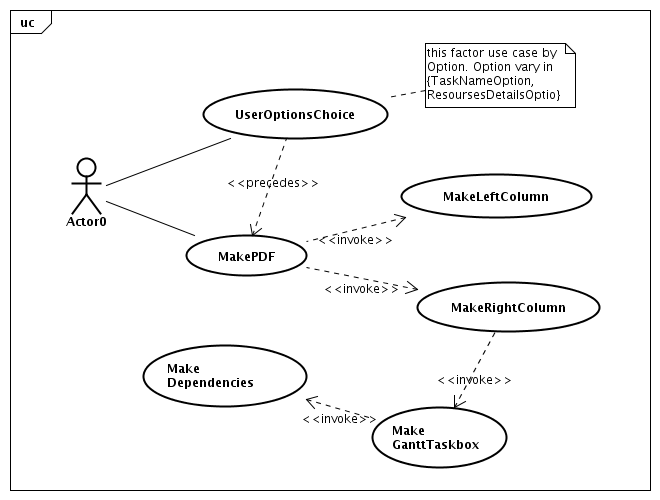
\includegraphics[width=0.8\textwidth]{Gantt/img/MakePDF.png} 
\end{figure}

\section{Make Left Column}
\label{seq:GanttMakeLeftColumn}
\subsection{Basic course}
Il client prende un reference al GanttChartGenerator e domanda la funzionalit\'a
per creare la colonna di sinistra del diagramma. \\
Il sistema costruisce una colonna di larghezza di dimensione \emph{fissa}.
Guarda se in UserOptionChoises \`e presente l'opzione TaskNameOption:
\begin{itemize}
  \item se \'e presente allora calcola la larghezza
\begin{displaymath}
	width_{nor}=lenght(max\lbrace id | \forall task: id =
WBS\_identifier(task) \rbrace) 
\end{displaymath}
dove la funzione $WBS\_identifier$ restituisce il WBS identifier relativo al 
parametro $task$ del dominio.

Poi $\forall task$ scrive $WBS\_identifier(task)$, un task per ogni riga.

\item altrimenti calcola
\begin{eqnarray}
width_{opt}=lenght(max\lbrace ::(id, task\_name) | \forall task: \\ id =
WBS\_identifier(task), \\ task\_name = Get\_TaskName(task)
\rbrace)
\end{eqnarray}
dove l'operatore $::$ concatena le stringhe passate come parametro, e
l'operatore \\$Get\_TaskName$ restituisce il nome del parametro
task.

Poi $\forall task$ scrive $::(WBS\_identifier(task), Get\_TaskName(task)$, un
task per ogni riga.
\end{itemize}

\subsection{Alternative course}
\begin{description}
\item[troncamento delle resourses] se $width_{opt} >
\frac{width_{diagram}}{6}$, con $width_{diagram}$ uguale alla larghezza totale
del diagramma, allora sia 
\begin{equation}cutted = cut(::(WBS\_identifier(task),
Get\_TaskName(task))\end{equation} 
la funzione $cut$ cancella caratteri in coda alla stringa in ingresso e
restituisce $cutted$, contenente i caratteri non cancellati, in modo che $cutted
= \frac{width_{diagram}}{6}-3$. \\ Il sistema scrive 
\begin{equation} 
::(cut(::(WBS\_identifier(task), Get\_TaskName(task)), ''\ldots'')
\end{equation}
\item[troncamento del WBS identifier] se avessi un identifier troppo lungo
dovrei fare lo stesso??
\end{description}
\section{Make GanttTaskbox}
\label{seq:makeGanttTaskbox}
\subsection{Basic course}
Il client prende un reference al GanttChartGenerator e domanda di creare la
rappresentazione grafica di un \emph{Task}. 

Il sistema esegue questi passi:
\begin{enumerate}
  \item recupera il \emph{Task} da rappresentare
  \item costruisce la rappresentazione grafica, il \emph{GanttTaskBox}
    in base alla scelta \emph{WBSTreeSpecification}.
  \item \`E possibile codificare delle informazioni aggiuntive:
    \begin{itemize}
   	  \item se \emph{UserOptionChoice} contiene \emph{ResourcesDetailsOption},
    	allora sul margine destro della \emph{GanttTaskBox} appendi la stringa
    	contenente la lista delle risorse cdns.
    	
    	Altrimenti appendi sul margine destro l'effort cdns.
    \end{itemize}
    
\end{enumerate}

\subsection{Alternative course}
\begin{description}
\item[troncamento delle resourses] se le informazioni testuali aggiuntive
superano la dimensione definita nel documento di specifica, allora si troncano
cdns.

\end{description}
\section{Make Right Column}
\label{seq:GanttRightRepresentation}
\subsection{Basic course}
Il client prende un reference al GanttChartGenerator e domanda di creare la
colonna di destra del diagramma. 

Il sistema esegue questi passi:
\begin{enumerate}
  \item costruisce una colonna di larghezza di dimensione \emph{fissa} che
  viene calcolata cdns.
  \item Il sistema effettua una ricerca per calcolare l'insieme dei \emph{Task}
  necessari da rappresentare nella colonna.
  \item Per ogni \emph{Task} trovato:
  \begin{itemize}
    \item invoca lo use case \ref{seq:makeGanttTaskbox}
    
    \item si posiziona il \emph{GanttTaskBox} creato nella giusta posizione
    temporale in base alla scelta \emph{TimeGrainOption}.
  \end{itemize}
  \item se \emph{UserOptionsChoice} contiene \emph{ShowDependencies} allora per
  ogni \emph{TaskBox} rappresentata, invoca lo use case 
  \ref{seq:makeDependencies}
\end{enumerate}

\subsection{Alternative course}
\begin{description}
\item[troncamento delle resourses] se le informazioni testuali aggiuntive
superano la dimensione definita nel documento di specifica, allora si troncano
cdns.

\end{description}
\section{Make PDF}
\label{seq:GanttMakePDF}

\subsection{Basic course}
Il client entra nella pagina relativa al diagramma Gantt e clicca sulla 
funzionalit\`a ''Make PDF''. Il sistema costruisce un oggetto in questo modo:
\begin{itemize}
  \item invoca lo use case \ref{seq:GanttMakeLeftColumn} per creare la
  colonna a sinistra.
  \item invoca lo use case \ref{seq:GanttRightRepresentation} per creare
  la rappresentazione nel tempo (colonna destra del diagramma).
\end{itemize}
Il sistema invio la pagina di risposta al client, aggiungendo accanto ai
pulsanti di reporting una icona per permettere il download del file generato.  

\subsection{Alternative course}
\begin{description}
\item[nessuna]
\end{description}



\end{document}